\clearpage
\section{Výpočty chlazení a výkonových ztrát}

\indent\indent Výpočet výkonové ztráty na LM317:
\begin{equation}
P_{LM317} = (V_i - V_o) \cdot I_o = (9 - 4,5) \cdot 0,5 = \underline{\underline{2,25~W}}
\nonumber
\end{equation}

Výpočet výkonové ztráty na schottkyho diodě:
\begin{equation}
P_{D} = V_F \cdot I_{OUT} \cdot \left(1-D_{(min)} \right) = 3 \cdot 0,455 \cdot (1-0,28) \doteq \underline{\underline{962~mW}}
\nonumber
\end{equation}

Výpočet výkonové ztráty na PFETu:
\begin{equation}
P_{PFET} = V_{IN_{(max)}} \cdot \left( Q_G \cdot F_S + I_{IN}\right) = 32 \cdot (24 \cdot 10^{-9} \cdot 300 \cdot 10^{3} + 1,3 \cdot 10^{-3}) = \underline{\underline{272~mW}}
\nonumber
\end{equation}

Výpočet celkového tepelného odporu chlazení LM317:
\begin{equation}
R_{thsys_{(LM317)}} = \dfrac{\vartheta_{j_{(max)}} - \vartheta_a}{P_{LM317}} = \dfrac{150 - 80}{2,25} \doteq \underline{\underline{32~KW^{-1}}}
\nonumber
\end{equation}

Výpočet celkového tepelného odporu chlazení schottkyho diody:
\begin{equation}
R_{thsys_{(D)}} = \dfrac{\vartheta_{j_{(max)}} - \vartheta_a}{P_{D}} = \dfrac{150 - 80}{0,962} \doteq \underline{\underline{73~KW^{-1}}}
\nonumber
\end{equation}

Výpočet celkového tepelného odporu chlazení PFETu:
\begin{equation}
R_{thsys_{(PFET)}} = \dfrac{\vartheta_{j_{(max)}} - \vartheta_a}{P_{PFET}} = \dfrac{175 - 80}{0,272} \doteq \underline{\underline{345~KW^{-1}}}
\nonumber
\end{equation}


\begin{figure}[H]
  \centering
  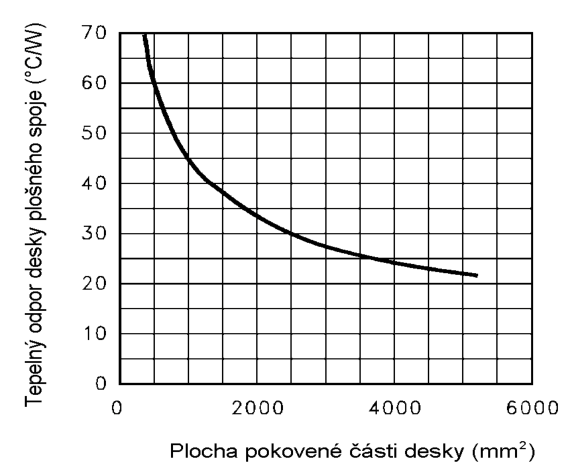
\includegraphics{img/DPS_odpor.pdf}
  \caption{Graf závislosti tepelného odporu plošného spoje na jeho ploše}
  \label{graf:1}
\end{figure}

Z grafů vyplývá, že shottkyho diodu a PFET nebude problém uchladit plošným spojem, pro LM317 ale vychází plocha mědi na můj vkus příliš veliká cca $7~cm \cdot 7~cm$ a tak zvolím klasické chlazení hliníkovým profilem. Vybral jsem chladič s tepelným odporem $11~KW^{-1}$, takže teplota křemíkového čipu LM317 by měla být nižší, než teplota maximální na kterou jsem počítal celkový tepelný odpor.